\section{Busca}

\begin{frame}{Busca em árvores binárias de busca}

	\begin{itemize}

        \item A busca em uma árvore binária de busca procura responder a seguinte questão:
            a informação $x$ está armazenada em algum dos nós da árvore?

        \item A importância desta operação nesta estrutura é tamanha que, de fato, a nomeia

        \item O algoritmo abaixo busca a informação $x$ em uma árvore binária de busca:

        \begin{enumerate}
            \item Começe no nó {raiz}

            \item Para cada nó {não nulo}:

            \begin{enumerate}
                \item Se $x$ {está} armazenado no nó, {retorne verdadeiro}

                \item Se $x$ for {menor} do que o valor 
                armazenado no nó, vá para a subárvore à {esquerda}

                \item Se $x$ for {maior} do que o valor 
                armazenado no nó, vá para a subárvore à {direita}
            \end{enumerate}

            \item Retorne falso
        \end{enumerate}

	\end{itemize}

\end{frame}

\begin{frame}[fragile]{Exemplo de busca em árvore binária de busca}

    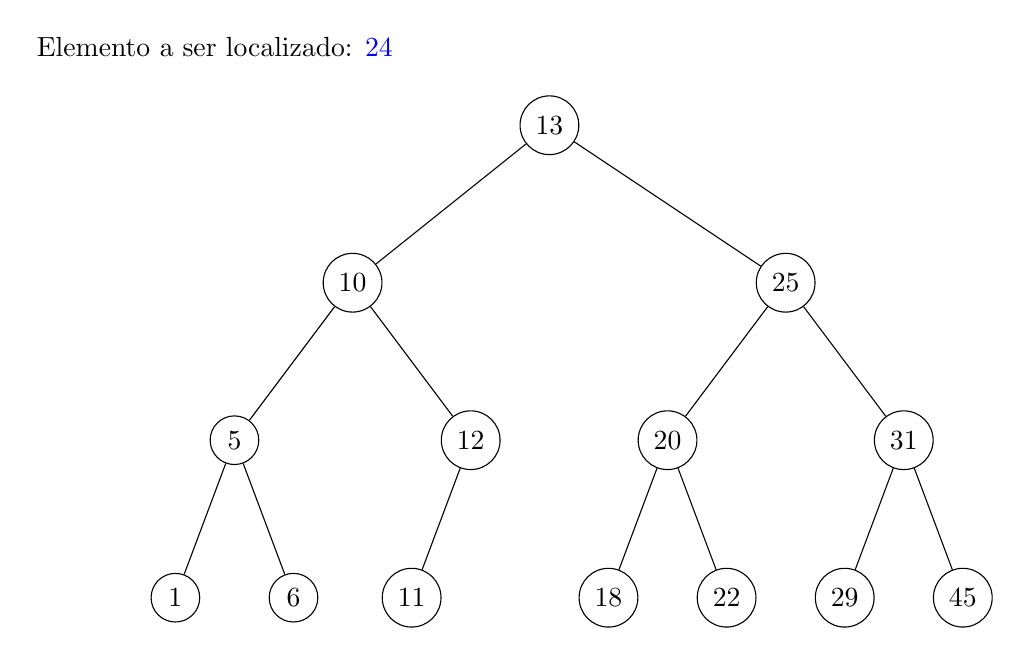
\begin{tikzpicture}

        \begin{scope}
            \node (X) at (2.5, 6) { Elemento a ser localizado: \textcolor{blue}{24}};

            \node[circle,draw] (A) at (6.75, 5) { $13$ };
            \node[circle,draw] (B) at (4.25, 3) { $10$ };
            \node[circle,draw] (C) at (9.75, 3) { $25$ };
            \node[circle,draw] (D) at (2.75, 1) { $5$ };
            \node[circle,draw] (E) at (5.75, 1) { $12$ };
            \node[circle,draw] (F) at (8.25, 1) { $20$ };
            \node[circle,draw] (G) at (11.25, 1) { $31$ };
            \node[circle,draw] (H) at (2, -1) { $1$ };
            \node[circle,draw] (I) at (3.5, -1) { $6$ };
            \node[circle,draw] (J) at (5, -1) { $11$ };
            \node[circle,draw] (L) at (7.5, -1) { $18$ };
            \node[circle,draw] (M) at (9, -1) { $22$ };
            \node[circle,draw] (N) at (10.5, -1) { $29$ };
            \node[circle,draw] (O) at (12, -1) { $45$ };

            \draw (A) -- (B);
            \draw (A) -- (C);
            \draw (B) -- (D);
            \draw (B) -- (E);
            \draw (C) -- (F);
            \draw (C) -- (G);

            \draw (D) -- (H);
            \draw (D) -- (I);
            \draw (E) -- (J);
            \draw (F) -- (L);
            \draw (F) -- (M);
            \draw (G) -- (N);
            \draw (G) -- (O);
        \end{scope}
    \end{tikzpicture}

\end{frame}

\begin{frame}[fragile]{Exemplo de busca em árvore binária de busca}

    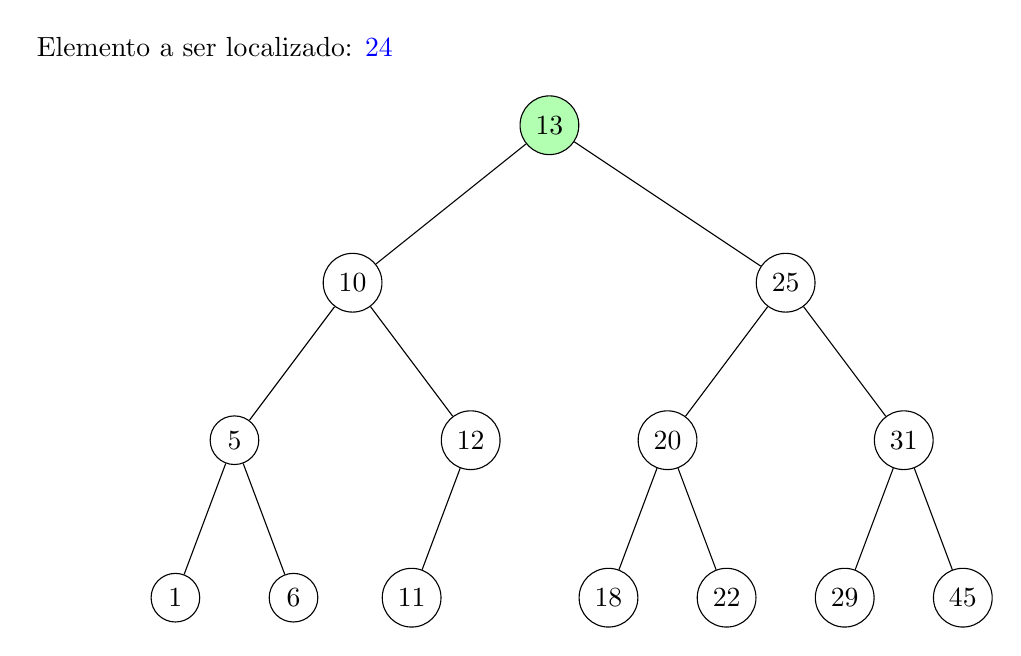
\begin{tikzpicture}

        \begin{scope}
            \node (X) at (2.5, 6) { Elemento a ser localizado: \textcolor{blue}{24}};

            \node[circle,draw,fill=green!30] (A) at (6.75, 5) { $13$ };
            \node[circle,draw] (B) at (4.25, 3) { $10$ };
            \node[circle,draw] (C) at (9.75, 3) { $25$ };
            \node[circle,draw] (D) at (2.75, 1) { $5$ };
            \node[circle,draw] (E) at (5.75, 1) { $12$ };
            \node[circle,draw] (F) at (8.25, 1) { $20$ };
            \node[circle,draw] (G) at (11.25, 1) { $31$ };
            \node[circle,draw] (H) at (2, -1) { $1$ };
            \node[circle,draw] (I) at (3.5, -1) { $6$ };
            \node[circle,draw] (J) at (5, -1) { $11$ };
            \node[circle,draw] (L) at (7.5, -1) { $18$ };
            \node[circle,draw] (M) at (9, -1) { $22$ };
            \node[circle,draw] (N) at (10.5, -1) { $29$ };
            \node[circle,draw] (O) at (12, -1) { $45$ };

            \draw (A) -- (B);
            \draw (A) -- (C);
            \draw (B) -- (D);
            \draw (B) -- (E);
            \draw (C) -- (F);
            \draw (C) -- (G);

            \draw (D) -- (H);
            \draw (D) -- (I);
            \draw (E) -- (J);
            \draw (F) -- (L);
            \draw (F) -- (M);
            \draw (G) -- (N);
            \draw (G) -- (O);
        \end{scope}
    \end{tikzpicture}

\end{frame}

\begin{frame}[fragile]{Exemplo de busca em árvore binária de busca}

    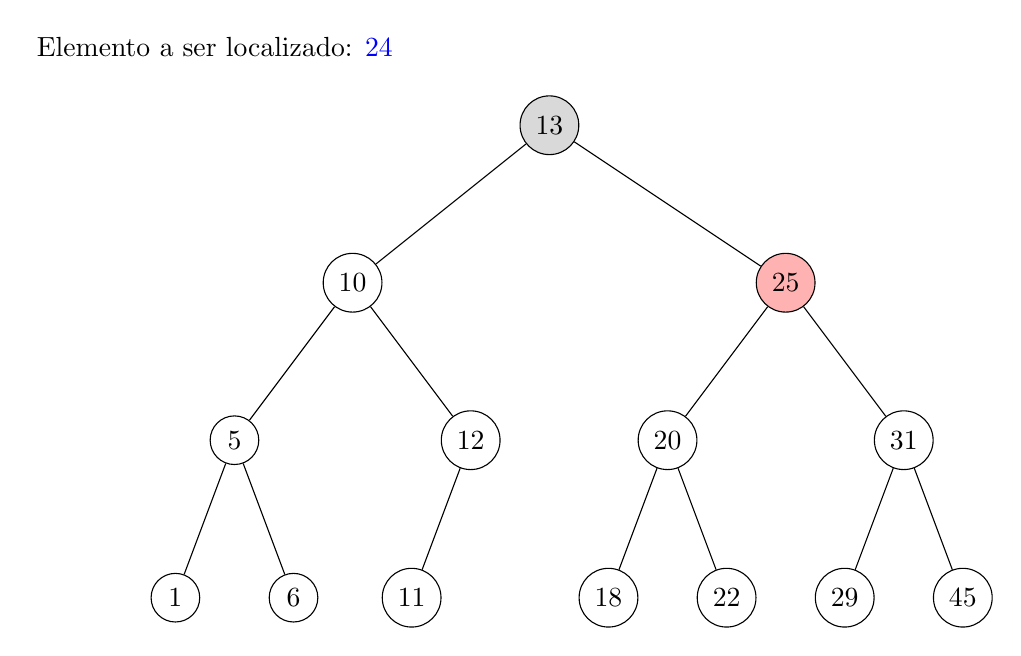
\begin{tikzpicture}

        \begin{scope}
            \node (X) at (2.5, 6) { Elemento a ser localizado: \textcolor{blue}{24}};

            \node[circle,draw,fill=gray!30] (A) at (6.75, 5) { $13$ };
            \node[circle,draw] (B) at (4.25, 3) { $10$ };
            \node[circle,draw,fill=red!30] (C) at (9.75, 3) { $25$ };
            \node[circle,draw] (D) at (2.75, 1) { $5$ };
            \node[circle,draw] (E) at (5.75, 1) { $12$ };
            \node[circle,draw] (F) at (8.25, 1) { $20$ };
            \node[circle,draw] (G) at (11.25, 1) { $31$ };
            \node[circle,draw] (H) at (2, -1) { $1$ };
            \node[circle,draw] (I) at (3.5, -1) { $6$ };
            \node[circle,draw] (J) at (5, -1) { $11$ };
            \node[circle,draw] (L) at (7.5, -1) { $18$ };
            \node[circle,draw] (M) at (9, -1) { $22$ };
            \node[circle,draw] (N) at (10.5, -1) { $29$ };
            \node[circle,draw] (O) at (12, -1) { $45$ };

            \draw (A) -- (B);
            \draw (A) -- (C);
            \draw (B) -- (D);
            \draw (B) -- (E);
            \draw (C) -- (F);
            \draw (C) -- (G);

            \draw (D) -- (H);
            \draw (D) -- (I);
            \draw (E) -- (J);
            \draw (F) -- (L);
            \draw (F) -- (M);
            \draw (G) -- (N);
            \draw (G) -- (O);
        \end{scope}
    \end{tikzpicture}

\end{frame}

\begin{frame}[fragile]{Exemplo de busca em árvore binária de busca}

    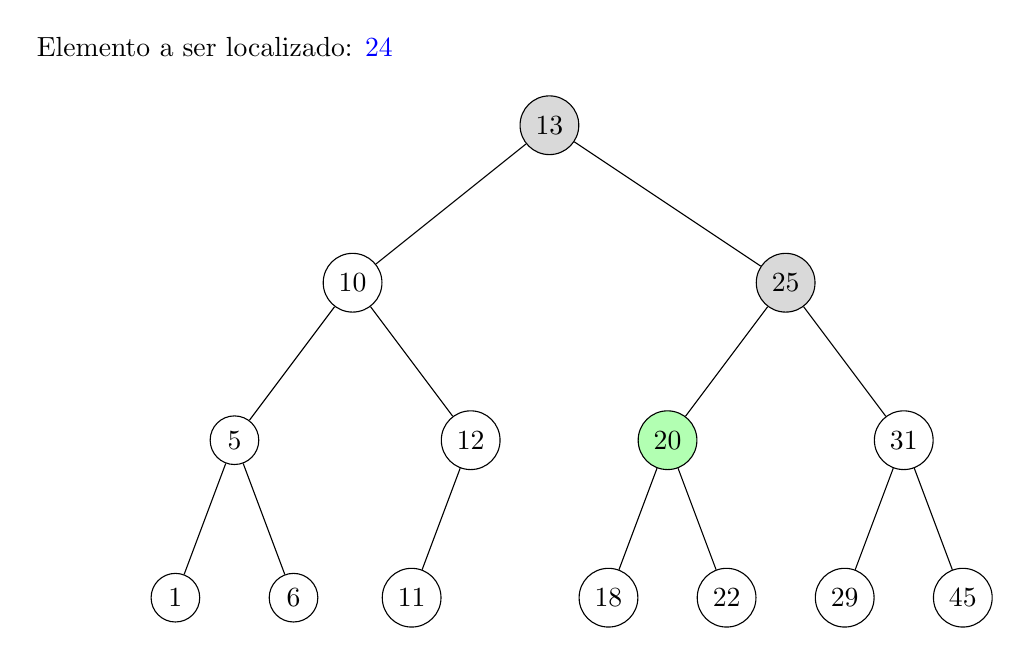
\begin{tikzpicture}

        \begin{scope}
            \node (X) at (2.5, 6) { Elemento a ser localizado: \textcolor{blue}{24}};

            \node[circle,draw,fill=gray!30] (A) at (6.75, 5) { $13$ };
            \node[circle,draw] (B) at (4.25, 3) { $10$ };
            \node[circle,draw,fill=gray!30] (C) at (9.75, 3) { $25$ };
            \node[circle,draw] (D) at (2.75, 1) { $5$ };
            \node[circle,draw] (E) at (5.75, 1) { $12$ };
            \node[circle,draw,fill=green!30] (F) at (8.25, 1) { $20$ };
            \node[circle,draw] (G) at (11.25, 1) { $31$ };
            \node[circle,draw] (H) at (2, -1) { $1$ };
            \node[circle,draw] (I) at (3.5, -1) { $6$ };
            \node[circle,draw] (J) at (5, -1) { $11$ };
            \node[circle,draw] (L) at (7.5, -1) { $18$ };
            \node[circle,draw] (M) at (9, -1) { $22$ };
            \node[circle,draw] (N) at (10.5, -1) { $29$ };
            \node[circle,draw] (O) at (12, -1) { $45$ };

            \draw (A) -- (B);
            \draw (A) -- (C);
            \draw (B) -- (D);
            \draw (B) -- (E);
            \draw (C) -- (F);
            \draw (C) -- (G);

            \draw (D) -- (H);
            \draw (D) -- (I);
            \draw (E) -- (J);
            \draw (F) -- (L);
            \draw (F) -- (M);
            \draw (G) -- (N);
            \draw (G) -- (O);
        \end{scope}
    \end{tikzpicture}

\end{frame}

\begin{frame}[fragile]{Exemplo de busca em árvore binária de busca}

    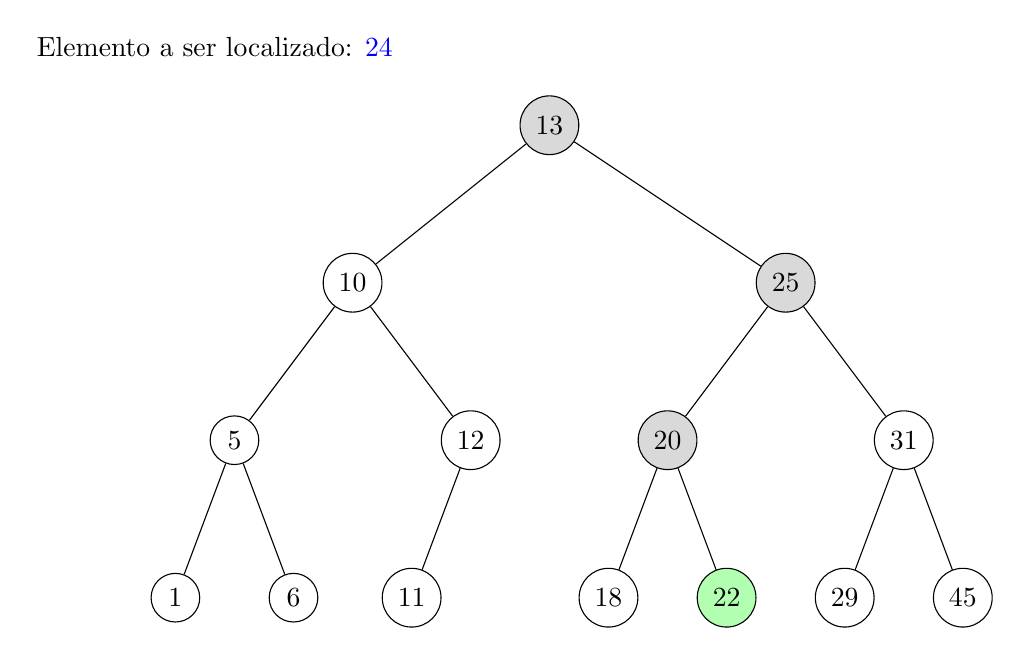
\begin{tikzpicture}

        \begin{scope}
            \node (X) at (2.5, 6) { Elemento a ser localizado: \textcolor{blue}{24}};

            \node[circle,draw,fill=gray!30] (A) at (6.75, 5) { $13$ };
            \node[circle,draw] (B) at (4.25, 3) { $10$ };
            \node[circle,draw,fill=gray!30] (C) at (9.75, 3) { $25$ };
            \node[circle,draw] (D) at (2.75, 1) { $5$ };
            \node[circle,draw] (E) at (5.75, 1) { $12$ };
            \node[circle,draw,fill=gray!30] (F) at (8.25, 1) { $20$ };
            \node[circle,draw] (G) at (11.25, 1) { $31$ };
            \node[circle,draw] (H) at (2, -1) { $1$ };
            \node[circle,draw] (I) at (3.5, -1) { $6$ };
            \node[circle,draw] (J) at (5, -1) { $11$ };
            \node[circle,draw] (L) at (7.5, -1) { $18$ };
            \node[circle,draw,fill=green!30] (M) at (9, -1) { $22$ };
            \node[circle,draw] (N) at (10.5, -1) { $29$ };
            \node[circle,draw] (O) at (12, -1) { $45$ };

            \draw (A) -- (B);
            \draw (A) -- (C);
            \draw (B) -- (D);
            \draw (B) -- (E);
            \draw (C) -- (F);
            \draw (C) -- (G);

            \draw (D) -- (H);
            \draw (D) -- (I);
            \draw (E) -- (J);
            \draw (F) -- (L);
            \draw (F) -- (M);
            \draw (G) -- (N);
            \draw (G) -- (O);
        \end{scope}
    \end{tikzpicture}

\end{frame}

\begin{frame}[fragile]{Exemplo de busca em árvore binária de busca}

    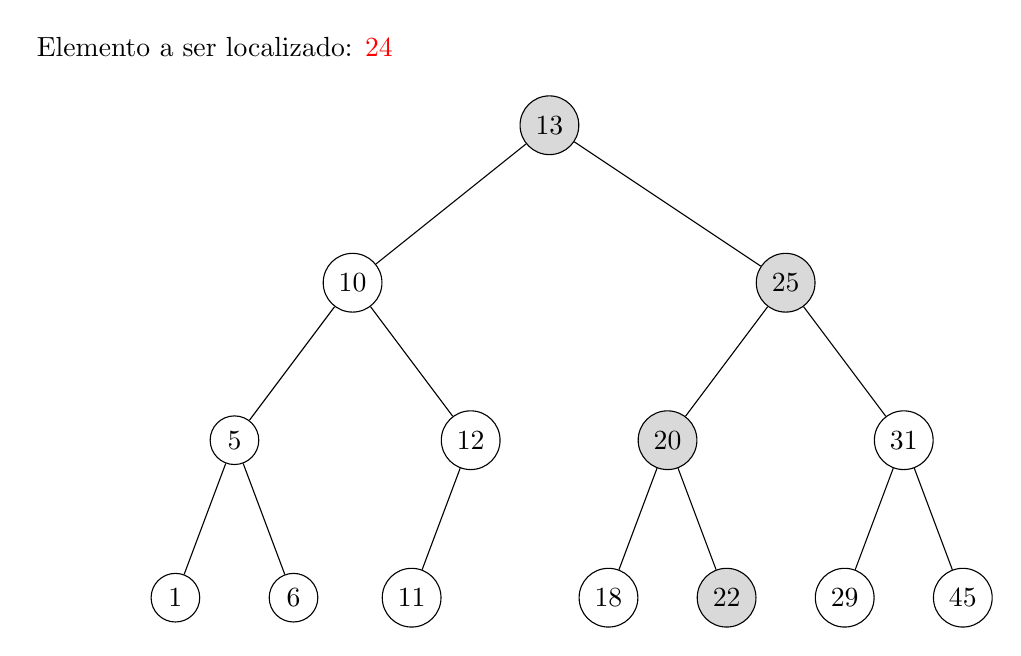
\begin{tikzpicture}

        \begin{scope}
            \node (X) at (2.5, 6) { Elemento a ser localizado: \textcolor{red}{24}};

            \node[circle,draw,fill=gray!30] (A) at (6.75, 5) { $13$ };
            \node[circle,draw] (B) at (4.25, 3) { $10$ };
            \node[circle,draw,fill=gray!30] (C) at (9.75, 3) { $25$ };
            \node[circle,draw] (D) at (2.75, 1) { $5$ };
            \node[circle,draw] (E) at (5.75, 1) { $12$ };
            \node[circle,draw,fill=gray!30] (F) at (8.25, 1) { $20$ };
            \node[circle,draw] (G) at (11.25, 1) { $31$ };
            \node[circle,draw] (H) at (2, -1) { $1$ };
            \node[circle,draw] (I) at (3.5, -1) { $6$ };
            \node[circle,draw] (J) at (5, -1) { $11$ };
            \node[circle,draw] (L) at (7.5, -1) { $18$ };
            \node[circle,draw,fill=gray!30] (M) at (9, -1) { $22$ };
            \node[circle,draw] (N) at (10.5, -1) { $29$ };
            \node[circle,draw] (O) at (12, -1) { $45$ };

            \draw (A) -- (B);
            \draw (A) -- (C);
            \draw (B) -- (D);
            \draw (B) -- (E);
            \draw (C) -- (F);
            \draw (C) -- (G);

            \draw (D) -- (H);
            \draw (D) -- (I);
            \draw (E) -- (J);
            \draw (F) -- (L);
            \draw (F) -- (M);
            \draw (G) -- (N);
            \draw (G) -- (O);
        \end{scope}
    \end{tikzpicture}

\end{frame}

\begin{frame}[fragile]{Implementação iterativa do algoritmo de busca}
    \inputsnippet{cpp}{1}{9}{codes/search.cpp}
\end{frame}

\begin{frame}[fragile]{Implementação iterativa do algoritmo de busca}
    \inputsnippet{cpp}{11}{30}{codes/search.cpp}
\end{frame}

\begin{frame}[fragile]{Notas sobre o algoritmo de busca}

	\begin{itemize}
		\item O algoritmo de busca em árvores binárias de busca também pode ser 
		implementado {recursivamente}:

        \inputcode{cpp}{codes/recursive_search.cpp}

		\item Uma {variante} do algoritmo retorna o ponteiro para  o elemento, se encontrado, 
            ou um ponteiro {nulo}, caso contrário

		\item A ordem de complexidade, no pior caso, é $O(N)$

		\item Em árvores balanceadas, o algoritmo é $O(\log N)$
	\end{itemize}

\end{frame}  

